% 2011 年辽宁卷理科第 22A 题：四点共圆与两割线。
% 来源 PDF：普通高考/2011/2011辽宁理.pdf，SHA-256 1fe81a3887c7782547f2dc987a468a7092be184781a1190af911ebb93a28e88e。
% 原页：第 2 页第 2 栏中部，书页码 682。示意。
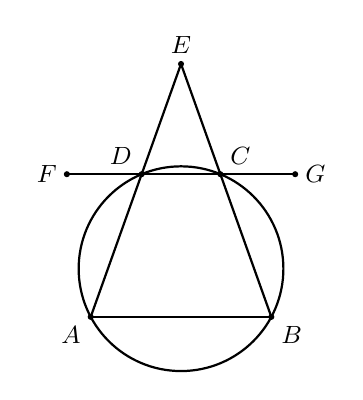
\begin{tikzpicture}[>=stealth, semithick, font=\small, scale=1.0]
  \draw[thick] (0,0) circle (1.3);
  \coordinate (E) at (0,2.6);
  \coordinate (D) at (-0.5,1.2);
  \coordinate (C) at (0.5,1.2);
  \coordinate (A) at (-1.147,-0.612);
  \coordinate (B) at (1.147,-0.612);
  \coordinate (F) at (-1.45,1.2);
  \coordinate (G) at (1.45,1.2);
  \draw[thick] (E)--(A);
  \draw[thick] (E)--(B);
  \draw[thick] (F)--(G);
  \draw (A)--(B);
  \fill (E) circle (1.1pt) node[above] {$E$};
  \fill (F) circle (1.1pt) node[left] {$F$};
  \fill (G) circle (1.1pt) node[right] {$G$};
  \fill (D) circle (1.1pt) node[above left] {$D$};
  \fill (C) circle (1.1pt) node[above right] {$C$};
  \fill (A) circle (1.1pt) node[below left] {$A$};
  \fill (B) circle (1.1pt) node[below right] {$B$};
\end{tikzpicture}
